\label{subsection_introspection}
\subsubsection{Cadre Général}

Le module d'introspection a pour objectif d'extraire, à partir des expériences passées de l'IA, de nouvelles formes remarquables potentiellement discriminantes pour les choix futurs. Pour ce faire, il choisi aléatoirement, en mémoire, au moins deux environnements ayant reçu une même annotation et tente d'étendre les formes déjà connues.

\paragraph{Exemple de la figure \ref{img_reco_forme_0}}
Nous considérons deux environnements présents en mémoire. Le premier décrit \emph{un homme avec un chapeau et un parapluie}, le second \emph{un homme avec un chapeau et une canne}. Nous souhaitons extraire de ces deux environnements la forme homme avec un chapeau. Pour ce faire, le module se base sur les connaissances relatives à ces environnements présentes en mémoire. Considérerons que \cogito{} sache déjà reconnaître un homme, le moteur d'introspection cherche alors à étendre le plus possible la forme \emph{homme} dans un des deux environnements tout en vérifiant que cette forme étendu peut être reconnue dans l'autre environnement, comme illustré dans la figure~\ref{img_reco_forme_injection}.

\begin{figure}[H] 
\begin{center}
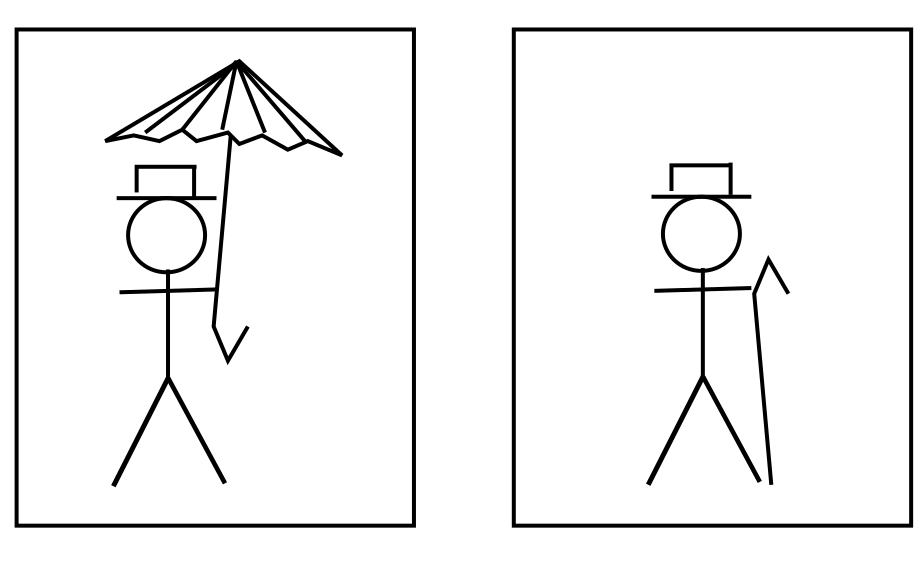
\includegraphics[width=0.8\textwidth]{files/raisonneur/reconnaissance_de_formes_0} 
\end{center}
\caption{Exemple d'environnements}
\label{img_reco_forme_0}
\end{figure}

\begin{figure}[H] 
\begin{center}
\includegraphics[width=0.8\textwidth]{files/raisonneur/reconnaissance_de_formes_injection} 
\end{center}
\caption{Exemple d'injection (basé sur la figure~\ref{img_reco_forme_0})}
\label{img_reco_forme_injection}
\end{figure}

\subsubsection{Application aux jeux de plateau}
\label{subsection_introspection_jeux}


La figure~\ref{img_cbs_reco0} représente, de façon graphique, le type d'environnement avec lequel doit travailler le moteur d'introspection.

\begin{figure}[H] 
\begin{center}
\includegraphics[width=0.7\textwidth]{files/raisonneur/cbs_reco0} 
\end{center}
\caption{Représentation graphique de l'environnement}
\label{img_cbs_reco0}
\end{figure}

Dans un premier temps, le moteur d'introspection va rechercher en mémoire deux plateaux ayant une même annotation et présentant des formes connues identiques (cf. figure~\ref{img_cbs_reco1}). Selon notre restriction aux jeux de plateaux, l'annotation peut être \og perdant \fg{} ou \og gagnant \fg{}.

\begin{figure}[H] 
\begin{center}
\includegraphics[width=0.7\textwidth]{files/raisonneur/cbs_reco1} 
\end{center}
\caption{Deux plateaux ayant des formes connues en commun} 
\label{img_cbs_reco1}
\end{figure}

Le module essaye ensuite d'étendre cette forme à partir d'un des plateaux tout en vérifiant qu'elle reste présente dans l'autre plateau, comme illustré dans la figure~\ref{img_cbs_reco_forme_injection}.

\begin{figure}[H] 
\begin{center}
\includegraphics[width=0.7\textwidth]{files/raisonneur/cbs_reco3} 
\end{center}
\caption{Illustration de l'injection sur des plateaux} 
\label{img_cbs_reco_forme_injection}
\end{figure}